\documentclass[fleqn,12pt]{olplainarticle}
% Use option lineno for line numbers 

%-----------------------------------------------
% Template by Eric Bojs, ebojs@kth.se
% Derived from KTHs template
%-----------------------------------------------

% Insert name, id and course codes here
\newcommand{\fullname}{Name McNameson}
\newcommand{\idnumber}{Id-number}
\newcommand{\courseid}{AA0000}
\newcommand{\coursename}{Course Name}
\newcommand{\githublink}{Githublink}



\title{\courseid : Homework X}
\author[1]{\fullname \ \idnumber}

\begin{abstract}
This report was written as the second assignment for the course \courseid \ \coursename for the fall/spring term 202X at KTH Kungliga Tekniska Högskolan. The report cannot be read independently; it is assumed that the reader has the project questions at hand. 

The code can be found at the following github repository: \href{\githublink}{HERE}.
\end{abstract}

\begin{document}

\flushbottom
\maketitle
\thispagestyle{empty}

\section*{Problem 1}
\subsection*{1.1}
\textit{Solution}
\begin{figure}[!h]
    \centering
        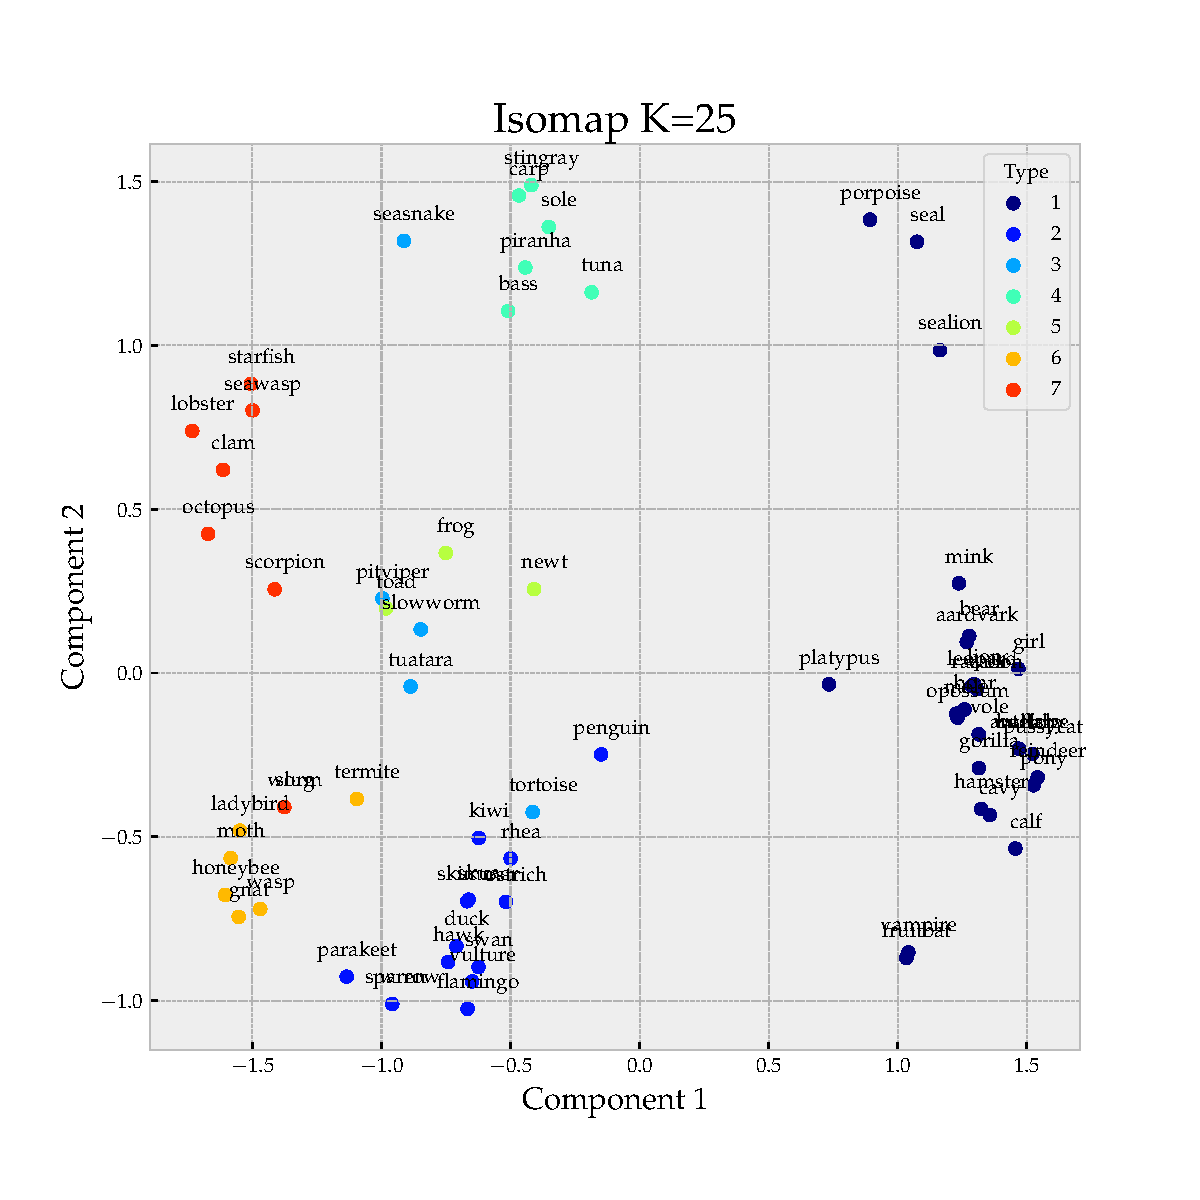
\includegraphics[width=12cm]{exampleFigure.pdf}
    \caption{Example figure}
    \label{exampleFigure}
\end{figure}

\end{document}